\chapter{RESULT OF MEASUREMENTS}\label{cha:result}
This chapter covers the results of the measurements described in~\chapterref{cha:measurements}. The first two sections cover the measurements made on the accelerometer and gyroscope sensor. Third section cover the result of the two camera measurements. This can be seen as one part of \textit{choose biometric characteristics} and also a part of \textit{choose features and matching algorithm}.

\section{Pre-measurements}
To get a hint if accelerometer were a possible fingerprinting candidate some pre-measurements were performed. This were in the early state of the development of the web-page used in measurements I and II. The measurement preformed on six different iPhones showed in~\figureref{fig:iPhoneScatter} indicates that the accelerometer is a sensor that may be good in fingerprinting purposes.
\begin{figure}[ht]
\centering
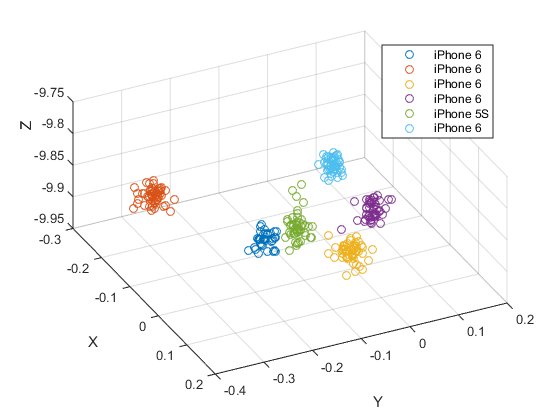
\includegraphics[scale=.6]{img/scatteriPhone}
\caption{Scatter-plot on accelerometer recordings of 6 Apple devices}
\label{fig:iPhoneScatter}
\end{figure}

\section{Result of measurements I  - Motion}\label{res:testI}
The data were gathered as described in~\sectionref{sec:measurementI} from the web-page in \figureref{fig:gyrotion} by spreading the the page. This resulted in over a hundred recordings with an FTE on 5\%, which had diversity in platforms, brands and models. Since the web-page where spread mostly to company employees the amount of devices with the same model is high as seen in ~\figureref{fig:measure1-topDevices}.
The purpose of this measurement where to identify if there were differences in terms of bias characteristics between the JavaScript's \texttt{accelerationIncludingGravity} and \texttt{acceleration}. The result of the measurements can be showed by making scatter-plots of the output acceleration of the devices. Shown in the ~\figureref{fig:measure1-topDevices} the \textit{Sony Xperia} devices represents more than a fifth of the total devices in the measurement. 
\begin{figure}[ht]
	\centering
	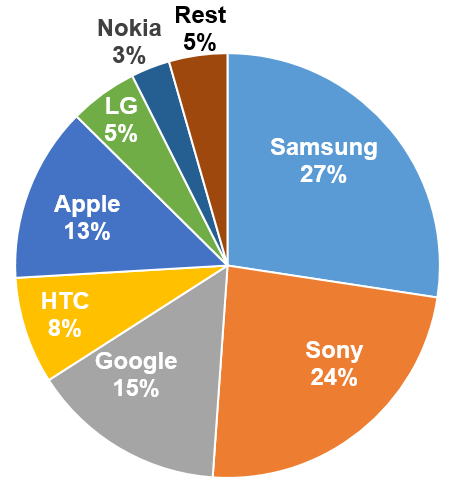
\includegraphics[scale=0.3]{img/measure1-brand}
	\caption{Diversity of device brand sampled in measurements I}
	\label{fig:measure1-brand}
\end{figure}
\begin{figure}[ht]
	\centering
	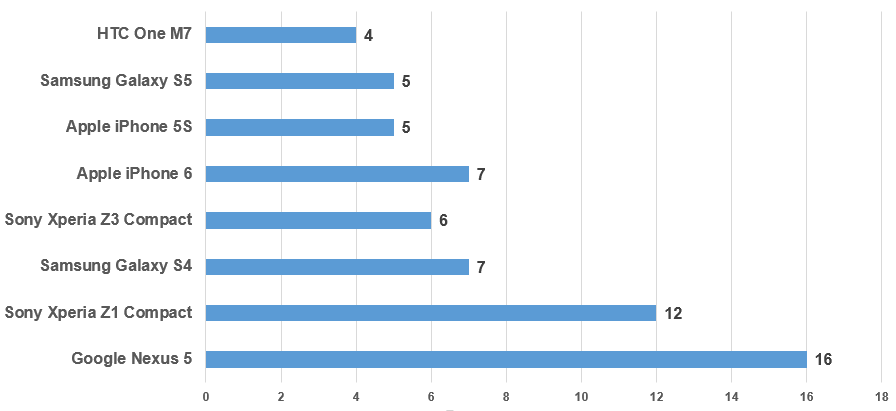
\includegraphics[scale=0.5]{img/measure1-devices}
	\caption{Most common devices models in measurements I}
	\label{fig:measure1-topDevices}
\end{figure}
The result of scatter-plots of measurements of 12 \textit{Sony Xperia} devices with and without gravity in accelerometer readings is shown in~\figureref{fig:scatter-withoutGrav} and~\figureref{fig:scatter-withGrav}.
\begin{figure}[ht]
	\centering
	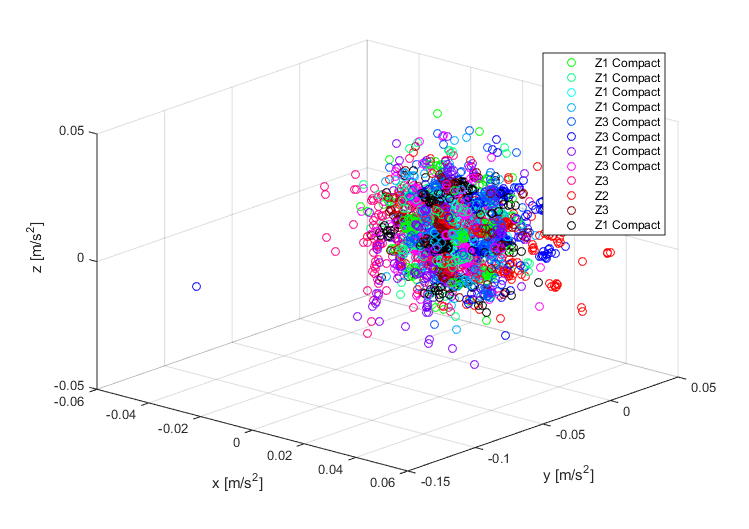
\includegraphics[scale=0.6]{img/res-measure1-scatter-notG}
	\caption{Bias from twelve \textit{Sony Xperia} devices measured with JavaScripts \texttt{acceleration}}
	\label{fig:scatter-withoutGrav}
\end{figure}
\begin{figure}[ht]
	\centering
	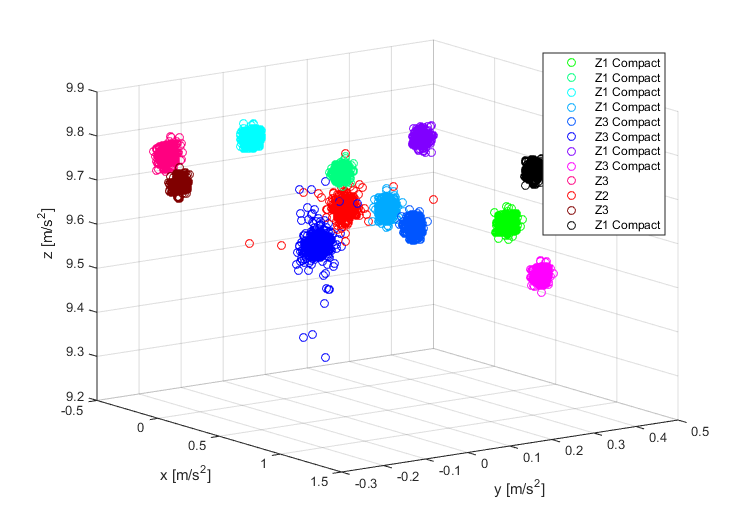
\includegraphics[scale=0.6]{img/res-measure1-scatter-inclG}
	\caption{Bias from twelve \textit{Sony Xperia} devices measured with JavaScripts \texttt{accelerationIncludingGravity}}
	\label{fig:scatter-withGrav}
\end{figure}

\section{Result of measurements II  - Motion}\label{res:testII}
The result here is an analyses of the gyroscope and accelerometer data collected from 60 devices with an FTE of 2\% by an improved version of the JavaScript web-page used in measurements I. The changes that were made is described in~\sectionref{sec:measurementII} to improve that analyze data. \\
The diversity of the devices brands in the measurement is shown in the~\figureref{fig:brandII} below. 
\begin{figure}[H]
	\centering
	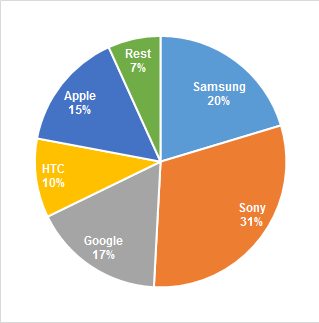
\includegraphics[scale=.4]{img/measure2-brands}
	\caption{Diversity of device brand sampled in measurements II}
	\label{fig:brandII}
\end{figure}

\subsection{Permanence of accelerometer}\label{sec:permanenceAcc}
When choosing biometric trait one of the factors is permanence described in \sectionref{auth:bio:character}, that is the trait not changing significantly over time. To test this measurement II were performed on a \textit{Sony Xperia Z1 Compact} over a period of 50 days. The choice of device was based on that \textit{Sony Xperia} devices is 30\% of the devices that data is collected from. The same test were also made on a \textit{Google Nexus 7} tablet. The graphs below shows the difference of accelerometer readings over time.
\begin{figure}[ht]
	\centering
	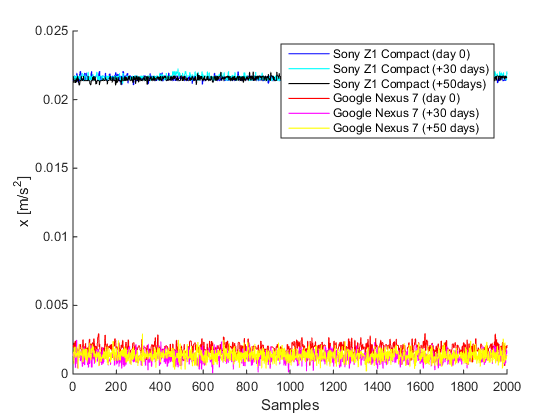
\includegraphics[scale=.7]{img/sensrec-nex-z1-acc-x}
	\caption{Accelerometer readings of x-axes on a  \textit{Sony Xperia Z1 Compact} and a \textit{Google Nexus 7} over 50 days}
	\label{fig:x50days}
\end{figure}
\begin{figure}[ht]
	\centering
	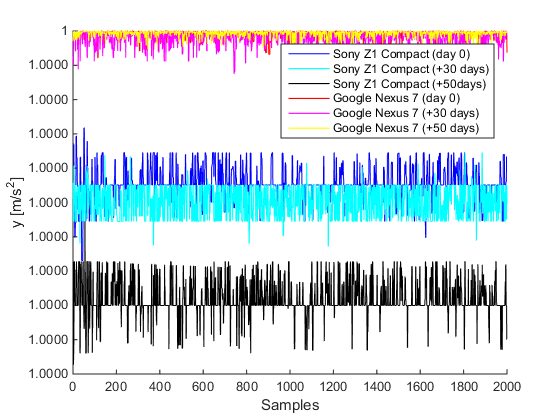
\includegraphics[scale=.7]{img/sensrec-nex-z1-acc-y}
	\caption{Accelerometer readings of y-axes on a  \textit{Sony Xperia Z1 Compact} and a \textit{Google Nexus 7} over 50 days}
	\label{fig:y50days}
\end{figure}
\begin{figure}[ht]
	\centering
	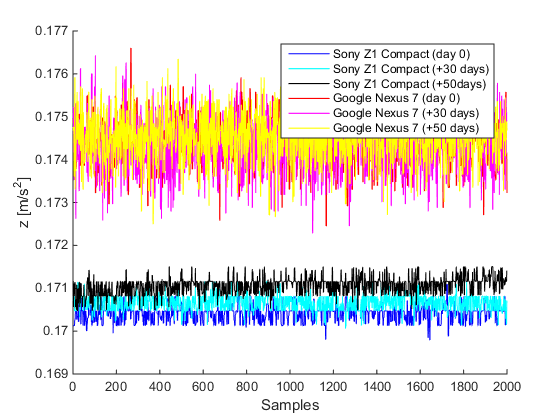
\includegraphics[scale=.7]{img/sensrec-nex-z1-acc-z}
	\caption{Accelerometer readings of z-axes on a  \textit{Sony Xperia Z1 Compact} and a \textit{Google Nexus 7} over 50 days}
	\label{fig:z50days}
\end{figure}
To get an perspective on this measurements among more devices the scatter-plot in~\figureref{fig:scatterSony50days} that include the same measurements from \textit{Sony Xperia Z1 Compact} as in~\figureref{fig:x50days},~\figureref{fig:y50days} and~\figureref{fig:z50days}.
\begin{figure}[ht]
	\centering
	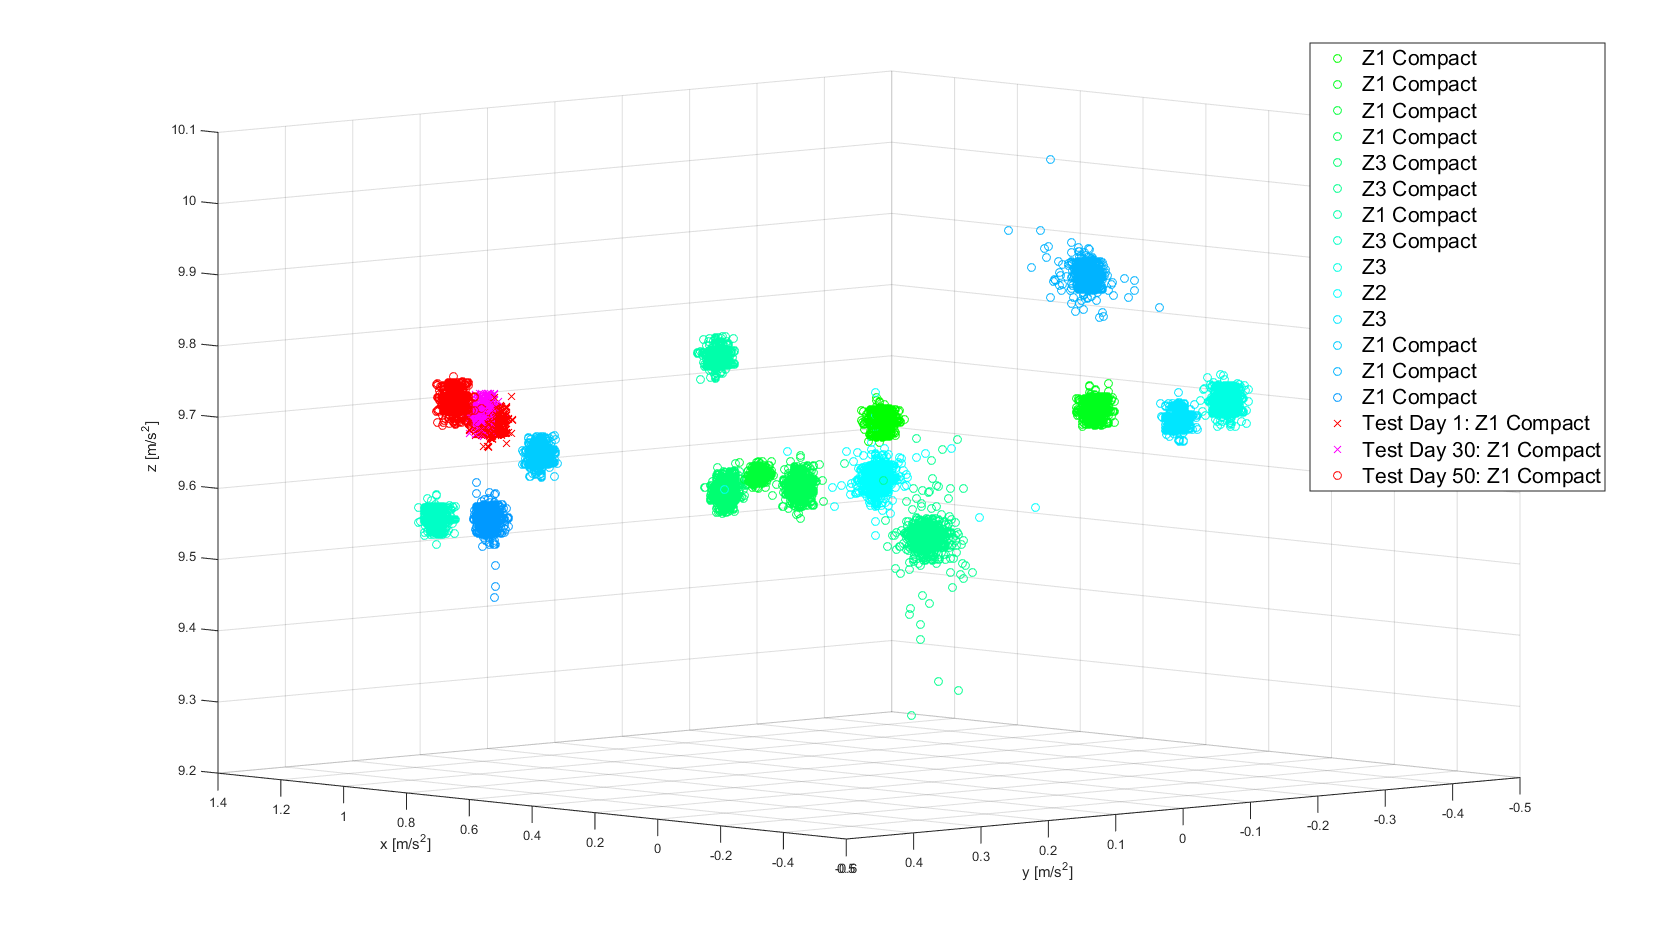
\includegraphics[scale=.3]{img/senrec-sony_scatter-2}
	\caption{Scatter-plot of accelerometer readings \textit{Sony Xperia}-device, one of them with measurements performed on the same device with 50 days apart.}
	\label{fig:scatterSony50days}
\end{figure} 

\subsection{Features of accelerometer data}\label{sec:featuresAcc}
As in ~\cite{sensor:accelPrint} I used statistical features calculated by the time domain. The features used and calculated as followed:
% === IfTime Gör en egen tabell!!
\begin{figure}[ht]
	\centering
	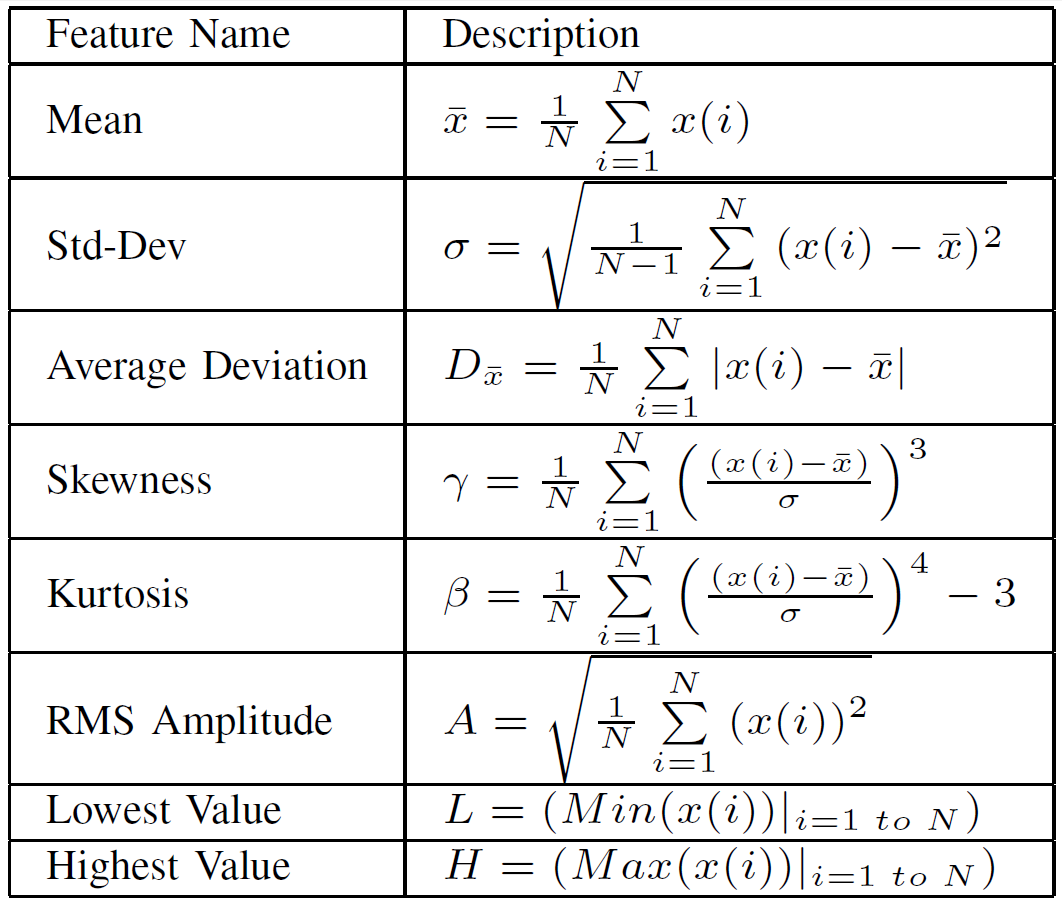
\includegraphics[scale=.35]{img/featureCalc}
	\caption{Calculations of statistical accelerometer features. \\\textit{From~\cite[p.6]{sensor:accelPrint}}}
	\label{fig:accFeatures}
\end{figure}
To compare these features and get a picture of if any of them are good for fingerprinting plots of devices were made. These can be found in~\appendixref{cha:matlabFeaturesPlot}. The chosen devices for the plots is the twelve \textit{Sony Xperia Z}-devices including the \textit{Sony Xperia Z1 Compact} that have measurements over 50 days. In these graphs it is possible to see that medium, min, max and the RMS paragraphs \textit{Sony Xperia Z1 Compact} measurements still are right gathered from the other device. Standard deviation looks to separate a bit more and kurtosis, and skewness means deviation looks nothing like being concerned.\\
In order to compare the properties that are best the distance between these points for all the 60 units were calculated. A point contain the x-, y- and z-coordinates of the feature and the distance is the Euclidean distance. From the distances are used so minimum and the median value from all the sample points calculated into features to compare with the same values calculated from only one unit (\textit{Sony Xperia Z1 Compact} or \textit{Google Nexus 7}) over time. The choice to use the median and not average value because it could be outliers in the measurements. Also adding the median as a feature since mean-value can be unreliable if there are outliers. As seen in~\tableref{tab:addlabel} the values strengthens the result read from~\appendixref{cha:matlabFeaturesPlot}.

\begin{table}[htbp]
  \centering
    \begin{tabular}{llrrrrr}
    \toprule
    \multicolumn{3}{l}{\textit{Minimum distance}} &       &       &       &  \\
          & Mean  & RMS   & Std.dev. & Min   & Max   & Median \\
    \midrule
    All   & 0,018 & 0,0193 & 0,0001 & 0,0287 & 0,0365 & 0 \\
    Z1Comp & 0,0171 & 0,0171 & 0,0002 & 0,0224 & 0,0144 & 0,0175 \\
          & 95\%  & 89\%  & 200\% & 78\%  & 39\%  &  \\
    Nexus7 & 0,0237 & 0,0182 & 0,0008 & 0,0267 & 0,0119 & 0,0225 \\
          & 132\% & 94\%  & 4\%   & 93\%  & 33\%  &  \\ 
    \toprule
    \multicolumn{3}{l}{\textit{Median distance}} &       &       &       &  \\
          & Mean  & RMS   & Std.dev. & Min   & Max   & Median \\
    \midrule
    All   & 0,7934 & 0,3925 & 0,0202 & 0,89  & 0,9199 & 0,7953 \\
    Z1Comp & 0,0519 & 0,0519 & 0,0009 & 0,0447 & 0,054 & 0,0575 \\
          & 7\%   & 13\%  & 690\% & 5\%   & 6\%   & 7\% \\
    Nexus7 & 0,0285 & 0,0275 & 0,0019 & 0,0361 & 0,0302 & 0,0283 \\
          & 4\%   & 7\%   & 10\%  & 4\%   & 3\%   & 4\% \\
    \bottomrule
    \end{tabular}%
    \caption{Comparing distance between values of statistical features for the accelerometer. \textit{Z1Comp} and \textit{Nexus7} is the devices that have been measured over 50 days. (\textit{Z1Comp}=\textit{Sony Xperia Z1 Compact} \& \textit{Nexus7}=\textit{Google Nexus 7})}
  \label{tab:addlabel}%
\end{table}%


\subsection{Gyroscope}
The same analysis of the measurement values as for the accelerometer has been done with the gyroscope. Since the output of the measurements is in degrees and as described in section~\ref{subsec:gyroJS} the alpha value goes from 0 to 360 degrees, beta from -180 to 180 degrees and gamma from -90 to 90 degrees. To get rid of the case when the values in measurement readings switch from 0 to 360 or -90 to 90. The output first is calculated trough sinus, cosine and tangent, ($\alpha=sin(alpha), \beta=cos(beta), \gamma=tan(gamma)$). As the measurements is in degrees the measurements is only the same if the device is rotated in the exactly same angular-values of the axes as last time. Constant bias cannot be calculated in the same way as for the accelerometer were the measurements should be zero without bias.\\
The constant bias from the gyroscope is calculated as the distance between the vectors ($v=\{\alpha, \beta,\gamma\}$) of the measurements, because that value would be the same in an ideal non-bias sensor.
That however didn't result in the same stability in permanence as seen in table~\ref{tab:featureGyro}.

% Table generated by Excel2LaTeX from sheet 'gyro'
\begin{table}[htbp]
  \centering
    \begin{tabular}{lrrrrr}
    \toprule
          & Mean  & Std.dev. & RMS   & Min   & Max \\
    \toprule
    \multicolumn{6}{l}{\textit{Minimum distance}} \\
    All   & 0,000188 & 1,31E-05 & 0,000112 & 2,63E-05 & 0 \\
    Z1Comp & 0,00924 & 0,001157 & 0,00896 & 0,009478 & 0,001348 \\
    Z1Comp/all & <<100\% & <<100\% & <<100\% & <<100\% &  \\
    Nexus7 & 0,006013 & 0,003204 & 0,006512 & 0,000738 & 0,000126 \\
    Nexus7/all & <<100\% & <<100\% & <<100\% & <<100\% &  \\
    \midrule
    \multicolumn{6}{l}{\textit{Median distance}} \\
    All   & 0,019079 & 0,005938 & 0,016074 & 0,012646 & 0,007945 \\
    Z1Comp & 0,00924 & 0,001157 & 0,00896 & 0,009478 & 0,001348 \\
    Z1Comp/all & 48\%  & 19\%  & 56\%  & 75\%  & 17\% \\
    Nexus7 & 0,006013 & 0,003204 & 0,006512 & 0,000738 & 0,000126 \\
    Nexus7/all & 32\%  & 54\%  & 41\%  & 6\%   & 2\% \\ \midrule
    %\multicolumn{6}{l}{\textit{Mean distance}} \\
    %All   & 0,037951 & 0,01339 & 0,037246 & 0,040401 & 0,02367 \\
    %Z1Comp & 0,00924 & 0,001157 & 0,00896 & 0,009478 & 0,001348 \\
    %Z1Comp/all & 24\%  & 9\%   & 24\%  & 23\%  & 6\% \\
    %Nexus7 & 0,006013 & 0,003204 & 0,006512 & 0,000738 & 0,000126 \\
    %Nexus7/all & 16\%  & 24\%  & 17\%  & 2\%   & 1\% \\ \midrule
    %\multicolumn{6}{l}{\textit{Maximum distance}} \\
    %All   & 0,403261 & 0,081063 & 0,313883 & 0,371617 & 0,157767 \\
    %Z1Comp & 0,00924 & 0,001157 & 0,00896 & 0,009478 & 0,001348 \\
    %Z1Comp/all & 2\%   & 1\%   & 3\%   & 3\%   & 1\% \\
    %Nexus7 & 0,006013 & 0,003204 & 0,006512 & 0,000738 & 0,000126 \\
    %Nexus7/all & 1\%   & 4\%   & 2\%   & 0\%   & 0\% \\
    \bottomrule
    \end{tabular}%
    \caption{Comparing distance between values of statistical features for the gyroscope. \textit{Z1Comp} and \textit{Nexus7} is the devices that have been measured over 50 days. (\textit{Z1Comp}=\textit{Sony Xperia Z1 Compact} \& \textit{Nexus7}=\textit{Google Nexus 7})}
  \label{tab:featureGyro}%
\end{table}%
If the gyroscope values in table~\ref{tab:featureGyro} are compared to the accelerometer values in~\ref{tab:addlabel}, is the accelerometer a much more stable over time. The percentage of the gyroscope distances is much higher than the accelerometer percentage.


\subsection{Allan variance}
As described in section~\ref{char:allan} the Allan variance is used to calibrate sensors. The Allan variance calculated from all sixty devices and compared in table~\ref{tab:allan} as the time features of the gyroscope and accelerometer. If the variance stays the same between measurements for each device it would be a good fingerprinting feature.\\
% Table generated by Excel2LaTeX from sheet 'allan'
\begin{table}[htbp]
  \centering
    \begin{tabular}{lrrrrr}
    \toprule
    \multicolumn{6}{l}{\textit{Minimum distance}} \\
          & All   & Z1Comp & Nexus7 & Z1C./All & Nex./All \\
          \midrule
    Accelerometer & 2,28E-14 & 9,06E-14 & 1,02E-12 & <<100\% & <<100\% \\
    Gyroscope & 1,91E-19 & 2,85E-17 & 2,57E-17 & <<100\% & <<100\% \\
    %Rotation rate & 2,55E-16 & 8,40E-15 & 2,67E-15 & <<100\% & <<100\% \\
    \toprule
    \multicolumn{6}{l}{\textit{Median distance}} \\
          & All   & Z1Comp & Nexus7 & Z1C./All & Nex./All \\
          \midrule
    Accelerometer & 3,64E-12 & 3,57E-13 & 4,96E-12 & 10\%  & < 100\% \\
    Gyroscope & 1,68E-16 & 4,17E-17 & 1,44E-16 & 25\%  & 86\% \\
    %Rotation rate & 8,25E-14 & 3,73E-11 & 3,18E-15 & <<100\% & 4\% \\
    \bottomrule
    \end{tabular}%
    \caption{The Allan variance differences between measurements of all devices and same devices (Z1Comp \& Nexus7)}
  \label{tab:allan}%
\end{table}%
As read from the table~\ref{tab:allan} isn't the Allan variance the same between measurements of the same device. Thus the variance between all the 60 devices is smaller than the variance between the variance of one device measured over time. This result does not make the Allan variance to a candidate of a fingerprinting feature for the motion sensors.  


\subsection{Simulate authentication of motion sensors in MATLAB}
To test that the features above is way of fingerprinting devices a simulation were performed in MATLAB. The concept is that a fingerprint of all devices is calculated. It contains the features described in~\sectionref{sec:featuresAcc} that resulted in the most stable values over time, thus min, max, mean and RMS. The code for making a fingerprint can be found in~\ref{cha:matlabAccSim} (listing~\ref{code:fingerprintCalc}).\\
\\
When a new measurement is sent in to the simulation, features are calculated and compared to the once already known devices. The comparing is done by an algorithm that calculates the point distance between all points of the input device and a known device. Point distance is the distance between two points. In this case all points of the input device is compared to all points in a known device. \\
The min, max, mean and RMS is then calculated between the distances. The smaller values the closer to the input device. 
The features is then used to decide if there is a match or not, by sorting out the smallest values. Since the percentage of features median distance for the accelerometer is around a twentieth a threshold of the 5\% the devices of each feature is chosen. If the most common device among the chosen devices is the input device there is a match. The code for the simulation can be found in~\ref{cha:matlabAccSim} (listing~\ref{code:fingerprintInput}).\\
As in biometric system the threshold decides how far from the values an input can be and sill be a match. This threshold creates a rate of match error in the system called FRR and FAR (see~\sectionref{sec:bio:measure}). There are two numbers that can be changed in the simulation that affects the error rates that is \texttt{th1} and \texttt{th2}. The result of these changed values is presented in table~\ref{tab:farfrr}.

\begin{table}[htbp]
  \centering
    \begin{tabular}{rrrrr}
    \toprule
    \textbf{FRR} & th1/th2 & 1     & 2     & 3 \\
    \midrule
          & 1     & 2,27\% & 8,62\% & 29,55\% \\
          & 2     & 20,45\% & 20,45\% & 29,55\% \\
          & 3     & 34,09\% & 34,09\% & 38,64\% \\
          &       &       &       &  \\
    \textbf{FAR} & th/F< & 1     & 2     & 3 \\
          & 1     & 0,00\% & 0,00\% & 0,00\% \\
          & 2     & 0,89\% & 0,45\% & 0,43\% \\
          & 3     & 1,77\% & 0,86\% & 0,44\% \\
    \bottomrule
    \end{tabular}%
    \caption{The FAR and FRR of the MATLAB simulation when changing threshold values \texttt{th1} and \texttt{th2} see appendix~\ref{cha:matlabAccSim}}
  \label{tab:farfrr}%
\end{table}%


% ========== CAMERA TEST ==========
\section{Result Camera-measurements}\label{sec:ResCam}
For the test of the camera sensor the PRNU value is calculated as an approximation of the algorithm described in section ~\ref{sec:measurement:camera} and also used by \cite{sensor:camera:DCIdent}. 

\subsection{Result of camera measurement I}
Since the purpose of this thesis compared to earlier work (section~\ref{earlier:camera}) has the purpose of authentication and not forensics, is convenience for the collecting and measurability a factor to take in account. That is why the first experiment is asked the users to record a 5 seconds video-clip with the device camera facing down on a flat object, like a table. Instead of making the user take 50 pictures or more which takes a lot of more time. \\
The video is then shuttled into images (100-200 from a 5 seconds video depending on fps on recording camera) that is used for calculating the PRNU. The MATLAB code for this is:\\
\lstinputlisting[caption={Shutter a video into picture, calculating the PRNU of the pictures in MATLAB},label={code:videoToPRNU},language=MATLAB]{code/video2prnu1.m}

To compare a pictures between all collected PRNU the same calculation to get the noise is done. Then the noise from the reference pictures is compared to all collected PRNU and correlation is calculated like the formula above in MATLAB:\\
\lstinputlisting[caption={Comparing the PRNU of an input picture with already known PRNU in MATLAB},label={code:PRNUinput},language=MATLAB]{code/corrCamTest1.m}

The result of identify an input PRNU with the PRNU from already known devices head a limit on only six devices there only two of them were correctly identified. Since~\cite{sensor:camera:DCIdent} made better result than this, the conclusion that the bad result were due to the use of video instead of pictures. Thus the decision to redo the measurements but with picture instead of videos for calculating the PRNU. 

\subsection{Result of camera measurement II}
Since the earlier test leaved out some of the PRNU noise when recorded a video instead of taking a picture the new test consist of 10 images from every device. The recommendation from \cite{sensor:camera:DCIdent} to use at least 50 images is here compensated by again using black images (picture taking with device camera facing down). Since the scene is always the same the noise removal will be better in fewer images. The same code is used as above with the different that the video to image step is removed. The sizes of the images in this case is better since the camera on the mobile devices by default uses higher resolution when taking a picture then when recording. \\
The result of this measurements started out good with none false match at five devices, but that number increased rapidly as you can see in table~\ref{tab:falseCam}. As the value grew that quickly no more samples from more devices were gathered.

% Table generated by Excel2LaTeX from sheet 'cam'
\begin{table}[htbp]
  \centering
    \begin{tabular}{rrr}
    \toprule
    Devices & FRR & Time [s] \\
    \midrule
    5     & 0\%   & 15-20s \\
    7     & 50\%  & 17-26s \\
    10    & 67\%  & 25-46s \\
    \bottomrule
    \end{tabular}%
    \caption{False rate and time taken to compare PRNU of camera images.}
  \label{tab:falseCam}%
\end{table}%


